
\documentclass[11pt]{article}
\usepackage[margin=1in]{geometry}
\usepackage[T1]{fontenc}
\usepackage[utf8]{inputenc}
\usepackage{lmodern}
\usepackage{microtype}
\usepackage[table]{xcolor}
\usepackage{amsmath,amssymb,amsfonts,mathtools,bm}
\IfFileExists{physics.sty}{%
  \usepackage{physics}%
}{%
  % Portable subset used by this project when the optional physics package
  % is not installed in the local TeX distribution.
  \NewDocumentCommand{\pdv}{o m m}{%
    \IfNoValueTF{##1}{\frac{\partial ##2}{\partial ##3}}%
    {\frac{\partial^{##1} ##2}{\partial ##3^{##1}}}%
  }
  \NewDocumentCommand{\dv}{o m m}{%
    \IfNoValueTF{##1}{\frac{\mathrm{d} ##2}{\mathrm{d} ##3}}%
    {\frac{\mathrm{d}^{##1} ##2}{\mathrm{d} ##3^{##1}}}%
  }
  \providecommand{\dd}{\mathop{}\!\mathrm{d}}
  \providecommand{\grad}{\nabla}
  \providecommand{\abs}[1]{\left\lvert ##1\right\rvert}
  \providecommand{\norm}[1]{\left\lVert ##1\right\rVert}
  \providecommand{\ket}[1]{\left\lvert ##1\right\rangle}
  \providecommand{\bra}[1]{\left\langle ##1\right\rvert}
}
\usepackage{booktabs,array,longtable,tabularx}
\usepackage{hyperref}
\usepackage{enumitem}
\usepackage{fancyhdr}
\usepackage{titlesec}
\usepackage{tcolorbox}
\usepackage{ragged2e}
\usepackage{setspace}
\IfFileExists{siunitx.sty}{%
  \usepackage{siunitx}%
}{%
  % Minimal text-safe fallback for the small number of \SI and \si calls in
  % this repository. Full siunitx formatting is used when available.
  \providecommand{\si}[1]{\ensuremath{\mathrm{##1}}}
  \providecommand{\SI}[2]{\ensuremath{##1\,\mathrm{##2}}}
}
\hypersetup{colorlinks=true, linkcolor=blue!50!black, urlcolor=blue!50!black, citecolor=blue!50!black}
\definecolor{TitleBlue}{HTML}{163A5F}
\definecolor{AccentTeal}{HTML}{2D6F73}
\definecolor{SoftBlue}{HTML}{EAF3F8}
\definecolor{SoftTeal}{HTML}{EDF8F6}
\definecolor{SoftGray}{HTML}{F5F7FA}
\definecolor{RuleGray}{HTML}{D7DEE8}
\pagestyle{fancy}
\fancyhf{}
\lhead{RadiationEffects\_proj2}
\rhead{Technical Notes}
\cfoot{\thepage}
\setlength{\headheight}{14pt}
\setlength{\parskip}{0.5em}
\setlength{\parindent}{0pt}
\onehalfspacing
\numberwithin{equation}{section}
\titleformat{\section}{\Large\bfseries\color{TitleBlue}}{\thesection}{0.6em}{}
\titleformat{\subsection}{\large\bfseries\color{AccentTeal}}{\thesubsection}{0.6em}{}
\titleformat{\subsubsection}{\normalsize\bfseries\color{TitleBlue}}{\thesubsubsection}{0.6em}{}
\newtcolorbox{overviewbox}{colback=SoftBlue,colframe=TitleBlue,boxrule=0.8pt,arc=2mm,left=3mm,right=3mm,top=2mm,bottom=2mm}
\newtcolorbox{physicsbox}{colback=SoftTeal,colframe=AccentTeal,boxrule=0.8pt,arc=2mm,left=3mm,right=3mm,top=2mm,bottom=2mm}
\newtcolorbox{notebox}{colback=SoftGray,colframe=AccentTeal,boxrule=0.6pt,arc=2mm,left=3mm,right=3mm,top=2mm,bottom=2mm}
\newcommand{\DocTitle}[3]{%
\begin{center}
{\LARGE \bfseries \color{TitleBlue} #1}\\[0.5em]
{\large \color{AccentTeal} #2}\\[0.8em]
{\normalsize #3}
\end{center}
\vspace{0.5em}}
\newenvironment{symtable}{\rowcolors{2}{SoftGray}{white}\begin{longtable}{>{\RaggedRight\arraybackslash}p{0.18\textwidth} >{\RaggedRight\arraybackslash}p{0.25\textwidth} >{\RaggedRight\arraybackslash}p{0.47\textwidth}}\toprule \textbf{Symbol / acronym} & \textbf{Name} & \textbf{Meaning in this document} \\ \midrule\endfirsthead\toprule \textbf{Symbol / acronym} & \textbf{Name} & \textbf{Meaning in this document} \\ \midrule\endhead}{\bottomrule\end{longtable}}


\newcommand{\ProjectTOC}{%
\vspace{0.6em}
{\hypersetup{linkcolor=TitleBlue,urlcolor=TitleBlue,citecolor=TitleBlue}\tableofcontents}
\vspace{1.0em}}

\newcommand{\SymbolsAcronymsSection}{%
\section*{Symbols and acronyms used in this document}%
\addcontentsline{toc}{section}{Symbols and acronyms used in this document}}

\newcommand{\rvec}{\bm{r}}
\newcommand{\qvec}{\bm{q}}
\newcommand{\nvec}{\bm{n}}
\newcommand{\xvec}{\bm{x}}
\newcommand{\kB}{k_{\mathrm{B}}}
\newcommand{\qp}{\mathrm{qp}}
\newcommand{\JJ}{\mathrm{JJ}}
\newcommand{\mfp}{\Lambda}
\allowdisplaybreaks

\usepackage{tikz}
\usetikzlibrary{arrows.meta,positioning,shapes.geometric,calc,decorations.pathmorphing}

\newcommand{\Om}{\Omega}
\newcommand{\Osub}{\Omega_{\mathrm{sub}}}
\newcommand{\Oox}{\Omega_{\mathrm{ox}}}
\newcommand{\Osc}{\Omega_{\mathrm{sc}}}
\newcommand{\Gint}{\Gamma_{\mathrm{int}}}
\newcommand{\Tph}{T_{\mathrm{ph}}}
\newcommand{\Tqp}{T_{\mathrm{qp}}}
\newcommand{\Tele}{T_{\mathrm{e}}}
\newcommand{\Tbath}{T_{\mathrm{bath}}}
\newcommand{\DeltaSC}{\Delta}
\newcommand{\Tc}{T_{\mathrm{c}}}
\newcommand{\kappaph}{\kappa_{\mathrm{ph}}}
\newcommand{\kappaqp}{\kappa_{\mathrm{qp}}}
\newcommand{\Cph}{C_{\mathrm{ph}}}
\newcommand{\Cqp}{C_{\mathrm{qp}}}
\newcommand{\nqp}{n_{\mathrm{qp}}}
\newcommand{\Npb}{N_{2\Delta}}
\newcommand{\Gqp}{G_{\mathrm{qp}}}
\newcommand{\Rqp}{R_{\mathrm{qp}}}
\newcommand{\betaPB}{\beta_{\mathrm{pb}}}
\newcommand{\tauesc}{\tau_{\mathrm{esc}}}
\newcommand{\tautrap}{\tau_{\mathrm{trap}}}
\newcommand{\taurec}{\tau_{\mathrm{rec}}}
\newcommand{\qdep}{\dot q_{\mathrm{dep}}}
\newcommand{\qpb}{\dot q_{\mathrm{pb}}}
\newcommand{\qrec}{\dot q_{\mathrm{rec}}}
\newcommand{\qesc}{\dot q_{\mathrm{esc}}}
\newcommand{\qtrap}{\dot q_{\mathrm{trap}}}
\renewcommand{\mfp}{\Lambda}
\newcommand{\Kn}{\mathrm{Kn}}
\newcommand{\vk}{v_{\mathrm{g}}}
\newcommand{\hK}{h_{\mathrm{K}}}
\newcommand{\RK}{R_{\mathrm{K}}}
\newcommand{\Gth}{G_{\mathrm{th}}}
\newcommand{\Edep}{E_{\mathrm{dep}}}
\newcommand{\Epb}{E_{\mathrm{pb}}}
\newcommand{\xiPB}{\eta_{\mathrm{pb}}}
\newcommand{\x}{\mathbf{x}}
\newcommand{\Jq}{\mathbf{q}}
\newcommand{\Jph}{\mathbf{q}_{\mathrm{ph}}}
\newcommand{\Jqp}{\mathbf{q}_{\mathrm{qp}}}
\newcommand{\nvecb}{\mathbf{n}}

\rhead{Module 4 superconductivity}
\begin{document}

\DocTitle{Module 4 Superconductivity Extension: Cryogenic Thermal Transport, Phonons, Quasiparticles, and Pair-Breaking Energy Flow}{How the preexisting ballistic-diffusive thermal module changes in the superconducting region}{Physics note for RadiationEffects\_proj2}

\begin{overviewbox}
\textbf{Purpose.} Module 4 originally described heat transport in a silicon-like device using continuum, ballistic-diffusive, and FEM thermal models. This superconductivity extension explains what changes when the same radiation-effects problem is moved to cryogenic superconducting-device operation. The essential change is not merely that the temperature is lower. The identity of the heat carriers changes. Normal electronic heat conduction is suppressed in superconducting films; substrate phonons can travel quasi-ballistically; interface thermal resistance can dominate; radiation-generated high-energy phonons can break Cooper pairs; and the most important device-level thermal state may be a nonequilibrium quasiparticle density rather than a single thermodynamic temperature. This note derives the required physics in a textbook style and translates it into Module 4 modeling requirements.
\end{overviewbox}

\ProjectTOC

\SymbolsAcronymsSection
\begin{symtable}
Module 4 & Thermal transport module & Existing module that evolves temperature or thermal energy after radiation energy deposition. \\
SC & Superconducting & State below a critical temperature where a condensate forms and electronic excitations are gapped. \\
QP & Quasiparticle & Broken-Cooper-pair excitation above the superconducting gap. \\
PBP & Pair-breaking phonon & Phonon with energy \(\hbar\omega \ge 2\Delta\), able to break a Cooper pair in a superconducting film. \\
RT & Rothwarf-Taylor model & Coupled rate model for quasiparticles and pair-breaking phonons. \\
BD & Ballistic-diffusive & Transport regime where some carriers fly ballistically while others scatter diffusively. \\
BTE & Boltzmann transport equation & Kinetic equation for distribution functions of phonons, quasiparticles, or other carriers. \\
Kapitza resistance & Thermal boundary resistance & Interface resistance that creates a temperature jump for a finite heat flux. \\
\(\x\) & Position & Spatial coordinate. \\
\(t\) & Time & Independent time coordinate. \\
\(T\) & Temperature & Thermodynamic temperature when local equilibrium is valid. \\
\(\Tph\) & Phonon temperature & Effective temperature of a phonon bath, if approximately thermal. \\
\(\Tqp\) & Quasiparticle temperature & Effective temperature of QPs, only meaningful if their distribution is quasi-thermal. \\
\(\Tbath\) & Bath temperature & Dilution-refrigerator or boundary temperature. \\
\(\Tc\) & Critical temperature & Temperature below which the superconducting condensate appears. \\
\(\DeltaSC\) & Superconducting gap & Minimum excitation energy for one quasiparticle; pair breaking needs roughly \(2\Delta\). \\
\(\Cph\) & Phonon heat capacity & Volumetric heat capacity of phonons. \\
\(\Cqp\) & Quasiparticle heat capacity & Electronic heat capacity associated with thermally excited QPs. \\
\(\kappaph\) & Phonon thermal conductivity & Conductivity of the phonon subsystem. \\
\(\kappaqp\) & Quasiparticle thermal conductivity & Conductivity of QPs in superconducting film. \\
\(\Jph\) & Phonon heat flux & Energy flux carried by phonons. \\
\(\Jqp\) & Quasiparticle heat flux & Energy flux carried by QPs. \\
\(\qdep\) & Deposited power density & Radiation or external heating source term. \\
\(\qpb\) & Pair-breaking power density & Energy transfer from pair-breaking phonons into QPs. \\
\(\qrec\) & Recombination power density & Energy released into phonons when QPs recombine. \\
\(\nqp\) & Quasiparticle density & Number of QPs per unit superconducting-film volume. \\
\(\Npb\) & Pair-breaking phonon population & Number density or effective population of phonons with \(\hbar\omega\ge 2\Delta\). \\
\(\Gqp\) & QP generation rate & Rate at which radiation, photons, or pair-breaking phonons create QPs. \\
\(\Rqp\) & QP recombination coefficient & Coefficient in the approximate quadratic recombination rate. \\
\(\betaPB\) & Pair-breaking coefficient & Rate coefficient for pair-breaking phonons creating QPs. \\
\(\tauesc\) & Escape/downconversion time & Time for high-energy phonons to leave or downconvert below pair-breaking energy. \\
\(\tautrap\) & Trap time & Characteristic time for QPs to be trapped or removed from the active film. \\
\(\hK\) & Kapitza conductance & Interface conductance per area. \\
\(\RK\) & Kapitza resistance & Inverse of Kapitza conductance per area. \\
\(\mfp\) & Mean free path & Average distance a heat carrier travels between scattering events. \\
\(\Kn\) & Knudsen number & Ratio \(\Kn=\mfp/L\), measuring ballistic character. \\
\(\Edep\) & Deposited energy & Energy deposited by one radiation event. \\
\(\xiPB\) & Pair-breaking efficiency & Fraction of deposited energy eventually creating QPs in a superconducting region. \\
\end{symtable}

\section{What Module 4 did before superconductivity}

The baseline Module 4 thermal problem starts from energy conservation. In the simplest continuum form, one evolves a temperature field \(T(\x,t)\) through
\begin{equation}
C(\x,T)\pdv{T}{t}=\nabla\cdot\left[k(\x,T)\nabla T\right]+\qdep(\x,t),
\label{eq:baseline_fourier}
\end{equation}
where \(C\) is volumetric heat capacity, \(k\) is thermal conductivity, and \(\qdep\) is the deposited power density from radiation or another source. This is the Fourier heat equation.

Module 4 already improved on a pure Fourier picture by allowing ballistic-diffusive physics. In the quasi-ballistic regime, the heat carrier mean free path \(\mfp\) is not small compared with the device length \(L\). The dimensionless measure is
\begin{equation}
\Kn=\frac{\mfp}{L}.
\end{equation}
When \(\Kn\ll 1\), a local temperature-gradient model is usually reasonable. When \(\Kn\sim 1\), heat flux is nonlocal and depends on carrier histories and boundaries.

A compact way to remember the baseline hierarchy is
\begin{align}
\text{microscopic:} \quad & \text{Boltzmann transport equation},\\
\text{quasi-ballistic reduced:} \quad & \text{ballistic-diffusive split},\\
\text{macroscopic limit:} \quad & \Jq=-k\nabla T. 
\end{align}
The original silicon-like Module 4 could still often be interpreted as a scalar thermal-energy model. The superconducting extension cannot.

\begin{physicsbox}
\textbf{Main transition.} Baseline Module 4 asks: how does a deposited heat source evolve into a temperature field? Superconducting Module 4 asks: how does deposited energy partition into substrate phonons, superconducting quasiparticles, pair-breaking phonons, interfaces, traps, and the cryogenic bath?
\end{physicsbox}

\section{The first correction: superconducting operation is not just low-temperature silicon}

A common modeling mistake is to take Eq.~\eqref{eq:baseline_fourier}, lower \(T\), insert temperature-dependent heat capacity and conductivity, and call the result a superconducting thermal model. That is insufficient for superconducting devices.

A realistic superconducting chip is a heterogeneous cryogenic structure:
\begin{enumerate}[label=\arabic*.]
\item a crystalline substrate such as Si or sapphire,
\item thin oxides and surface dielectric layers,
\item superconducting films such as Al, Nb, TiN, NbTiN, or related materials,
\item Josephson junction barriers,
\item normal-metal traps, ground planes, packaging layers, wirebonds, and interfaces,
\item a dilution refrigerator bath connected through weak thermal paths.
\end{enumerate}
The heat carriers are material-dependent. In the substrate, low-temperature heat is usually carried mainly by phonons. In a normal metal, electrons can dominate. In a superconductor well below \(\Tc\), the condensate carries charge and supercurrent but carries essentially no entropy in equilibrium; thermal electronic excitations are exponentially suppressed except for nonequilibrium quasiparticles.

\begin{figure}[h]
\centering



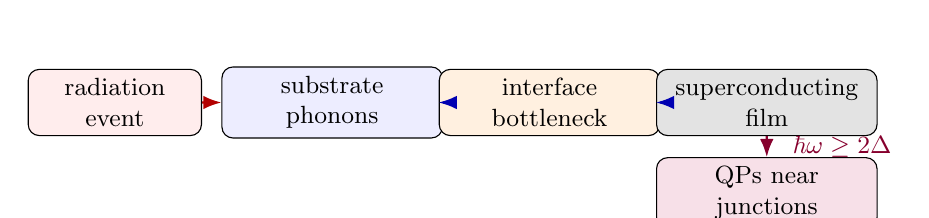
\begin{tikzpicture}[scale=0.92,every node/.style={font=\small}]
\node[draw,rounded corners,fill=red!7,align=center,minimum width=2.2cm,minimum height=0.75cm] (rad) at (0,1.6) {radiation\\event};
\node[draw,rounded corners,fill=blue!7,align=center,minimum width=2.8cm,minimum height=0.75cm] (sub) at (3.0,1.6) {substrate\\phonons};
\node[draw,rounded corners,fill=orange!12,align=center,minimum width=2.8cm,minimum height=0.75cm] (int) at (6.0,1.6) {interface\\bottleneck};
\node[draw,rounded corners,fill=gray!22,align=center,minimum width=2.8cm,minimum height=0.75cm] (film) at (9.0,1.6) {superconducting\\film};
\node[draw,rounded corners,fill=purple!12,align=center,minimum width=2.8cm,minimum height=0.75cm] (qp) at (9.0,0.35) {QPs near\\junctions};
\draw[-{Latex[length=2.3mm]},thick,red!70!black] (rad) -- (sub);
\draw[-{Latex[length=2.3mm]},thick,blue!70!black] (sub) -- (int);
\draw[-{Latex[length=2.3mm]},thick,blue!70!black] (int) -- (film);
\draw[-{Latex[length=2.3mm]},thick,purple!70!black] (film) -- node[right,xshift=2mm]{\(\hbar\omega\ge2\Delta\)} (qp);
\end{tikzpicture}
\caption{Superconducting Module 4 must track energy flow across subsystems. A substrate energy deposition creates a nonlocal phonon burst; pair-breaking phonons impinging on superconducting films create quasiparticles; interfaces and traps control relaxation to the bath.}
\label{fig:sc_module4_stack}
\end{figure}

\section{Thermal carriers below the superconducting transition}

\subsection{Phonons}

Phonons remain a primary heat carrier in substrates and dielectrics. At low temperatures, the phonon heat capacity of a crystalline dielectric follows approximately the Debye law
\begin{equation}
\Cph(T) \approx \beta_D T^3,
\label{eq:debye_C}
\end{equation}
where \(\beta_D\) depends on density, sound velocities, and the Debye temperature. If boundary scattering limits the mean free path, the phonon thermal conductivity scales roughly as
\begin{equation}
\kappaph \sim \frac{1}{3}\Cph v_s \mfp_{\mathrm{ph}} \propto T^3,
\label{eq:phonon_kappa_lowT}
\end{equation}
provided \(\mfp_{\mathrm{ph}}\) is temperature-independent and geometry-limited.

This low-temperature scaling has a major implication: small deposited energies can create large transient temperature excursions because \(\Cph\) is tiny. But the word ``temperature'' must be used carefully. Immediately after radiation energy deposition, the phonon distribution is not necessarily thermal. A high-energy phonon population can propagate ballistically and interact with superconducting films before downconverting to a thermal phonon bath.

\subsection{Electrons in a normal metal}

In a normal metal, electronic heat capacity and thermal conductivity are often approximated by
\begin{equation}
C_e \approx \gamma T,
\qquad
\kappa_e \approx L_0 \sigma T,
\label{eq:normal_metal_electrons}
\end{equation}
where \(\gamma\) is the Sommerfeld coefficient and \(L_0\) is the Lorenz number. This channel is important in normal-metal traps and wiring.

\subsection{Electrons in a superconductor}

In a BCS superconductor below \(\Tc\), electronic excitations require energy at least \(\Delta\). The equilibrium quasiparticle density is approximately exponentially suppressed:
\begin{equation}
\nqp^{\mathrm{eq}}(T) \sim 2N_0\sqrt{2\pi k_B T\Delta}\exp\left(-\frac{\Delta}{k_B T}\right),
\label{eq:nqp_eq}
\end{equation}
where \(N_0\) is the single-spin density of states at the Fermi level in the normal state. The electronic heat capacity of the superconducting excitations is likewise exponentially suppressed at \(T\ll\Tc\):
\begin{equation}
\Cqp(T) \propto \exp\left(-\frac{\Delta}{k_B T}\right)
\quad \text{up to algebraic prefactors.}
\label{eq:Cqp_exp}
\end{equation}
Therefore, simply using normal-state electronic thermal conductivity inside a superconducting film is wrong. The condensate does not provide ordinary thermal conduction because it is a coherent ground-state component with no entropy. Heat in the superconducting film is carried by QPs and phonons, not by the condensate as a normal electron gas.

\begin{notebox}
At millikelvin temperatures, equilibrium theory may predict an extremely small \(\nqp\), but experiments often observe nonequilibrium QP populations much larger than equilibrium values. This is why Module 4 should include nonequilibrium QP generation and removal channels rather than relying only on \(\Cqp(T)\).
\end{notebox}

\section{Energy gap and the pair-breaking threshold}

The superconducting energy gap is the energetic separation between the condensate ground state and quasiparticle excitations. A single QP has energy at least \(\Delta\) above the condensate. Breaking one Cooper pair creates two QPs, so the threshold energy is
\begin{equation}
E_{\mathrm{threshold}} \approx 2\Delta.
\label{eq:pair_breaking_threshold}
\end{equation}
A phonon or photon with energy \(\hbar\omega\ge2\Delta\) can in principle break a Cooper pair. The corresponding threshold frequency is
\begin{equation}
f_{2\Delta}=\frac{2\Delta}{h}.
\end{equation}
For weak-coupling BCS superconductors near zero temperature, a useful estimate is
\begin{equation}
2\Delta(0) \approx 3.52 k_B\Tc.
\label{eq:bcs_gap}
\end{equation}
The exact value depends on material, disorder, film thickness, and strong-coupling effects.

The key Module 4 implication is that energy deposited into the substrate does not need to produce a high local temperature in order to damage a superconducting qubit. It can produce a nonthermal phonon population whose high-energy tail breaks Cooper pairs in remote superconducting electrodes.

\section{Why one temperature field is insufficient}

\subsection{Local equilibrium assumption}

A temperature field is meaningful when the local distribution of the relevant carriers is close to equilibrium. For phonons, this means the phonon occupation approximately follows a Bose-Einstein distribution at some \(T\). For electrons or QPs, it means a Fermi-Dirac-like distribution with a meaningful effective temperature.

Radiation events violate this assumption. Immediately after deposition, energy may be stored in electron-hole pairs, optical phonons, acoustic phonons, QPs, high-energy photons, and local defect excitations. These components do not necessarily equilibrate on the same timescale.

A better superconducting Module 4 state is therefore a vector of fields, for example
\begin{equation}
\mathbf{u}(\x,t)=
\begin{bmatrix}
u_{\mathrm{ph,sub}}(\x,t) \\
u_{\mathrm{ph,film}}(\x,t) \\
 n_{\mathrm{qp}}(\x,t) \\
 n_{2\Delta}(\x,t)
\end{bmatrix},
\label{eq:state_vector}
\end{equation}
where \(u_{\mathrm{ph,sub}}\) is substrate phonon energy density, \(u_{\mathrm{ph,film}}\) is film phonon energy density, \(n_{\mathrm{qp}}\) is QP density, and \(n_{2\Delta}\) is a population or energy density of pair-breaking phonons.

\subsection{Near-equilibrium two-temperature approximation}

If the phonon and QP distributions are each internally close to equilibrium but not mutually equilibrated, a two-temperature model may be used:
\begin{align}
\Cqp(\Tqp)\pdv{\Tqp}{t}
&=\nabla\cdot\left[\kappaqp(\Tqp)\nabla\Tqp\right]
-\Sigma_{\mathrm{qp-ph}}(\Tqp,\Tph)+S_{\mathrm{qp}},
\label{eq:twoT_qp}\\
\Cph(\Tph)\pdv{\Tph}{t}
&=\nabla\cdot\left[\kappaph(\Tph)\nabla\Tph\right]
+\Sigma_{\mathrm{qp-ph}}(\Tqp,\Tph)+S_{\mathrm{ph}}.
\label{eq:twoT_ph}
\end{align}
This form is useful, but only when an effective QP temperature exists. For sparse nonequilibrium QPs generated by radiation, a density-based kinetic model is often more physical.

\section{Radiation energy partition in a superconducting chip}

A radiation event from Module 1 provides a deposited energy map. In a warm semiconductor model, Module 4 may convert this into heat generation. In a superconducting chip, the energy goes through a cascade:
\begin{enumerate}[label=\arabic*.]
\item primary energy deposition in substrate, film, oxide, or package;
\item creation of electron-hole pairs, hot electrons, or local excitations;
\item emission and downconversion of high-energy phonons;
\item ballistic or quasi-ballistic propagation of phonons through the substrate;
\item absorption of phonons in superconducting films;
\item pair breaking when \(\hbar\omega\ge2\Delta\);
\item QP diffusion, trapping, recombination, and phonon re-emission;
\item final escape to the bath through interfaces, wiring, phonon traps, and package paths.
\end{enumerate}

A minimal energy-partition rule can be written as
\begin{equation}
\Edep = E_{\mathrm{thermal\;ph}}+E_{2\Delta}+E_{\mathrm{qp}}+E_{\mathrm{trap}}+E_{\mathrm{defect}}+E_{\mathrm{escape}},
\label{eq:partition}
\end{equation}
where \(E_{2\Delta}\) is energy in pair-breaking phonons and \(E_{\mathrm{qp}}\) is energy stored in QPs.

For a reduced model, define a pair-breaking efficiency \(\xiPB\):
\begin{equation}
E_{\mathrm{qp,created}} \approx \xiPB E_{\mathrm{dep,reachable}},
\label{eq:pair_efficiency}
\end{equation}
where \(E_{\mathrm{dep,reachable}}\) is the portion of the deposited energy that reaches superconducting films as sufficiently energetic phonons or photons. Then the initial number of created QPs is roughly
\begin{equation}
N_{\mathrm{qp,0}}\approx \frac{E_{\mathrm{qp,created}}}{\Delta}.
\label{eq:Nqp_from_energy}
\end{equation}
The denominator is \(\Delta\), not \(2\Delta\), because the created energy is stored in individual quasiparticles after pair breaking. In practice, losses and excess energies modify the estimate.

\section{Phonon transport: diffusive, ballistic, and boundary-limited}

\subsection{Phonon Boltzmann equation}

Let \(f_\lambda(\x,\mathbf{k},t)\) be the occupation of a phonon mode \(\lambda\) with wave vector \(\mathbf{k}\), frequency \(\omega_{\lambda\mathbf{k}}\), and group velocity \(\mathbf{v}_{\lambda\mathbf{k}}\). The phonon BTE is
\begin{equation}
\pdv{f_\lambda}{t}+\mathbf{v}_{\lambda\mathbf{k}}\cdot\nabla_{\x} f_\lambda
=\left(\pdv{f_\lambda}{t}\right)_{\mathrm{coll}}+s_\lambda.
\label{eq:phonon_bte}
\end{equation}
Under the relaxation-time approximation,
\begin{equation}
\left(\pdv{f_\lambda}{t}\right)_{\mathrm{coll}}=-\frac{f_\lambda-f_\lambda^{0}(T)}{\tau_\lambda},
\label{eq:phonon_rta}
\end{equation}
where \(f^0\) is the local equilibrium Bose-Einstein distribution.

The phonon energy density and flux are
\begin{align}
u_{\mathrm{ph}} &= \sum_\lambda \int \hbar\omega_{\lambda\mathbf{k}} f_\lambda D_\lambda(\mathbf{k})\,d\mathbf{k},\\
\Jph &= \sum_\lambda \int \hbar\omega_{\lambda\mathbf{k}} \mathbf{v}_{\lambda\mathbf{k}} f_\lambda D_\lambda(\mathbf{k})\,d\mathbf{k}.
\end{align}
A diffusive closure gives \(\Jph=-\kappaph\nabla\Tph\), but a superconducting chip after radiation often starts in a nonlocal ballistic regime.

\subsection{Ballistic-diffusive split for superconducting Module 4}

The existing Module 4 ballistic-diffusive idea remains valuable, but the carrier is now often substrate phonons rather than a generic heat field. Write
\begin{equation}
f_{\mathrm{ph}}=f_{\mathrm{b}}+f_{\mathrm{m}},
\end{equation}
where \(f_{\mathrm{b}}
\) is a boundary- or event-originating ballistic component and \(f_{\mathrm{m}}\) is a scattered medium component. At the energy-density level,
\begin{equation}
u_{\mathrm{ph}} = u_{\mathrm{b}} + u_{\mathrm{m}},
\qquad
\Jph=\Jq_{\mathrm{b}}+\Jq_{\mathrm{m}}.
\end{equation}
The diffusive part satisfies a conservation equation such as
\begin{equation}
\pdv{u_{\mathrm{m}}}{t}+\nabla\cdot\Jq_{\mathrm{m}}
= Q_{\mathrm{scatter\;from\;b}}+Q_{\mathrm{internal}}-Q_{\mathrm{to\;film}}-Q_{\mathrm{escape}}.
\label{eq:um_sc}
\end{equation}
The ballistic part should be attenuated along rays with mean free path \(\mfp_{\mathrm{ph}}(\omega,T,\mathrm{surface})\). A reduced ray expression is
\begin{equation}
I_{\mathrm{b}}(s,\omega,\hat\Omega,t)
=I_{\mathrm{src}}(s_0,\omega,\hat\Omega,t-s/v_g)
\exp\left[-\int_{s_0}^{s}\frac{ds'}{\mfp_{\mathrm{ph}}(\omega,s')}\right].
\label{eq:ballistic_ray_sc}
\end{equation}
This form is especially relevant because pair-breaking depends strongly on whether high-frequency phonons reach superconducting electrodes before losing energy below \(2\Delta\).

\section{Interface thermal resistance and Kapitza boundaries}

At cryogenic temperatures, interfaces often dominate thermal relaxation. Across an interface \(\Gamma_{12}\) between materials 1 and 2, the heat flux is not necessarily continuous with a continuous temperature. Instead,
\begin{equation}
\Jq_1\cdot\nvecb = \hK(T_1,T_2)(T_1-T_2)
=\Jq_2\cdot\nvecb,
\label{eq:kapitza_linear}
\end{equation}
for a linearized interface law. Equivalently,
\begin{equation}
T_1-T_2=\RK \left(\Jq\cdot\nvecb\right),
\qquad \RK=\frac{1}{\hK}.
\label{eq:kapitza_R}
\end{equation}
For phonon-dominated interfaces, the conductance is often strongly temperature dependent. A common low-temperature scaling is
\begin{equation}
\frac{P}{A}=\alpha_K\left(T_1^4-T_2^4\right),
\label{eq:kapitza_T4}
\end{equation}
which linearizes near \(T_0\) to
\begin{equation}
\hK(T_0)=4\alpha_KT_0^3.
\label{eq:kapitza_linearized}
\end{equation}
The details depend on acoustic mismatch, diffuse mismatch, roughness, contamination, passivation, film thickness, and interface disorder.

\begin{physicsbox}
\textbf{Module 4 implication.} In superconducting operation, boundary conditions can be as important as the bulk PDE. A model with accurate \(\kappaph\) but no Kapitza interface terms may predict unrealistically fast cooling.
\end{physicsbox}

\section{Quasiparticle kinetics and the Rothwarf-Taylor model}

\subsection{Why QP density is a thermal variable}

For superconducting qubits, the relevant thermal damage metric is often not the phonon temperature but the density of nonequilibrium QPs near Josephson junctions. QPs provide dissipation channels and can degrade qubit coherence. A thermal module for superconducting operation should therefore evolve \(\nqp(\x,t)\) or provide source terms to a QP module.

\subsection{Minimal QP diffusion-recombination equation}

A reduced spatial QP model is
\begin{equation}
\pdv{\nqp}{t}
=\nabla\cdot\left(D_{\mathrm{qp}}\nabla\nqp\right)
+G_{\mathrm{qp}}(\x,t)
-R_{\mathrm{qp}}\left(\nqp^2-(n_{\mathrm{qp}}^{\mathrm{eq}})^2\right)
-\frac{\nqp}{\tautrap}.
\label{eq:qp_diff_rec}
\end{equation}
Here \(D_{\mathrm{qp}}\) is QP diffusivity, \(G_{\mathrm{qp}}\) is generation from pair-breaking phonons or photons, the quadratic term models recombination, and \(\tautrap\) captures trapping or loss to engineered normal-metal traps.

The energy density stored in near-gap QPs is approximately
\begin{equation}
u_{\mathrm{qp}}\approx \Delta \nqp,
\label{eq:uqp_nqp}
\end{equation}
when most QPs are near the gap edge. A more detailed model must integrate over the QP energy distribution.

\subsection{Rothwarf-Taylor equations}

The Rothwarf-Taylor model captures the bottleneck between QPs and high-energy phonons. In a simple spatially local form,
\begin{align}
\dv{\nqp}{t} &= G + 2\betaPB \Npb - R\nqp^2 - \frac{\nqp}{\tautrap},
\label{eq:RT_qp}\\
\dv{\Npb}{t} &= \frac{1}{2}R\nqp^2 - \betaPB\Npb - \frac{\Npb}{\tauesc}+G_{2\Delta}.
\label{eq:RT_ph}
\end{align}
The terms have direct meanings:
\begin{itemize}
\item \(G\): direct QP generation;
\item \(2\betaPB\Npb\): pair-breaking phonons create two QPs per broken pair;
\item \(R\nqp^2\): two QPs recombine into a Cooper pair;
\item \(\frac{1}{2}R\nqp^2\): recombination creates one high-energy phonon per pair;
\item \(\tauesc\): high-energy phonons escape, downconvert, or leave the active volume.
\end{itemize}

The RT model is essential because recombination does not necessarily remove pair-breaking energy. Recombination emits a phonon with energy of order \(2\Delta\). If that phonon remains in the film, it can break another Cooper pair. This is the phonon bottleneck.

\subsection{Spatially extended RT model}

For Module 4, spatial transport should be included:
\begin{align}
\pdv{\nqp}{t}
&=\nabla\cdot(D_{\mathrm{qp}}\nabla\nqp)+G+2\betaPB\Npb-R\nqp^2-\frac{\nqp}{\tautrap},
\label{eq:spatial_RT_qp}\\
\pdv{\Npb}{t}
&=\nabla\cdot(D_{2\Delta}\nabla\Npb)+\frac{1}{2}R\nqp^2-\betaPB\Npb-\frac{\Npb}{\tauesc}+G_{2\Delta}.
\label{eq:spatial_RT_ph}
\end{align}
A fully kinetic model would replace \(D_{2\Delta}\) with ballistic phonon transport, but Eq.~\eqref{eq:spatial_RT_ph} is a useful reduced starting point.

\section{Energy conservation with QPs and phonons}

The QP and pair-breaking phonon equations must be coupled to energy conservation. Multiplying Eq.~\eqref{eq:spatial_RT_qp} by \(\Delta\) gives an approximate near-gap QP energy equation. The pair-breaking phonon energy density is roughly
\begin{equation}
u_{2\Delta}\approx 2\Delta \Npb.
\end{equation}
Ignoring transport and trap loss for a moment, the RT pair-breaking and recombination terms exchange energy internally. Pair breaking transfers \(2\Delta\) from one phonon to two QPs. Recombination transfers energy from two QPs back to one phonon. Thus a consistent energy model should satisfy
\begin{equation}
\left.\pdv{}{t}(\Delta\nqp+2\Delta\Npb)\right|_{\mathrm{pb+rec}}
\approx 0,
\end{equation}
up to excess energies and downconversion losses. This conservation check is one of the most important numerical tests.

For a multi-field energy model,
\begin{align}
\pdv{u_{\mathrm{ph}}}{t} + \nabla\cdot\Jph
&= \qdep - \qpb + \qrec -\qesc,\\
\pdv{u_{\mathrm{qp}}}{t} + \nabla\cdot\Jqp
&= \qpb - \qrec - \qtrap,
\end{align}
where \(\qpb\), \(\qrec\), and \(\qtrap\) must be defined consistently with the rate equations.

\section{Superconducting heat capacity and thermal conductivity}

\subsection{Substrate and dielectric regions}

For insulating substrates and dielectrics at low temperature,
\begin{equation}
C_{\mathrm{sub}}(T)\approx \beta_D T^3,
\qquad
\kappa_{\mathrm{sub}}(T)\approx \frac{1}{3}C_{\mathrm{sub}}v_s\mfp_{\mathrm{eff}}.
\end{equation}
The effective mean free path may be limited by sample dimensions, surfaces, defects from Module 3, or isotope/disorder scattering:
\begin{equation}
\frac{1}{\mfp_{\mathrm{eff}}}
=\frac{1}{\mfp_{\mathrm{boundary}}}
+\frac{1}{\mfp_{\mathrm{defect}}}
+\frac{1}{\mfp_{\mathrm{isotope}}}
+\frac{1}{\mfp_{\mathrm{anharmonic}}}.
\label{eq:matthiessen_ph}
\end{equation}
This is the thermal-coupling point between Module 3 and Module 4: cryogenic defect populations may be immobile, but they still scatter phonons and modify \(\kappaph\).

\subsection{Superconducting film regions}

In superconducting film regions, the thermal conductivity has multiple components:
\begin{equation}
\kappa_{\mathrm{sc}} = \kappa_{\mathrm{ph,film}} + \kappa_{\mathrm{qp}} + \kappa_{\mathrm{other}}.
\end{equation}
The QP contribution is suppressed relative to the normal state when the QP density is near equilibrium. A practical reduced model may use
\begin{equation}
\kappaqp(\x,t) \approx \frac{1}{3} C_{\mathrm{qp,eff}}(\x,t)v_{\mathrm{qp}}\ell_{\mathrm{qp}},
\end{equation}
where \(C_{\mathrm{qp,eff}}\) is inferred from the actual \(\nqp\), not from equilibrium \(T\) alone. If one uses an effective QP temperature, then \(C_{\mathrm{qp}}(T)\) should have superconducting exponential suppression.

\section{Cryogenic boundary conditions}

\subsection{Bath boundary}

A boundary connected to the dilution refrigerator should rarely be modeled as a perfect Dirichlet temperature unless the thermal link is much stronger than all internal impedances. A more physical boundary condition is
\begin{equation}
-\Jq\cdot\nvecb = h_{\mathrm{bath}}(T,\Tbath)(T-\Tbath),
\label{eq:bath_robin}
\end{equation}
or the nonlinear phonon form
\begin{equation}
-\Jq\cdot\nvecb = \alpha_{\mathrm{bath}}(T^4-\Tbath^4).
\end{equation}

\subsection{Superconducting film-substrate interface}

At a substrate-film interface, the heat flux from substrate phonons into the film is
\begin{equation}
\Jph^{\mathrm{sub}}\cdot\nvecb = h_{\mathrm{sub-sc}}(\Tph^{\mathrm{sub}}-\Tph^{\mathrm{film}}),
\label{eq:sub_sc_interface}
\end{equation}
for the thermal phonon part. The pair-breaking part should be treated separately:
\begin{equation}
G_{\mathrm{qp}}^{\mathrm{film}}(\x,t)
= \int_{\omega\ge2\Delta/\hbar}
\eta_{\mathrm{abs}}(\omega,\x)\Phi_{\mathrm{ph}}(\omega,\x,t)\,d\omega,
\label{eq:Gqp_pair_breaking_flux}
\end{equation}
where \(\Phi_{\mathrm{ph}}\) is the incident phonon flux and \(\eta_{\mathrm{abs}}\) is an absorption/pair-breaking probability.

This distinction matters. A low-energy thermal phonon flux heats the film. A high-energy pair-breaking phonon flux directly creates QPs even if the thermal temperature rise is small.

\section{Connection to the existing ballistic-diffusive Module 4}

The existing Module 4 can be reused, but its variables must be reinterpreted. The warm-device variable \(T\) becomes only one part of a multi-carrier picture.

\begin{center}
\rowcolors{2}{SoftGray}{white}
\begin{tabularx}{0.96\textwidth}{>{\RaggedRight\arraybackslash}p{0.30\textwidth}>{\RaggedRight\arraybackslash}p{0.30\textwidth}>{\RaggedRight\arraybackslash}X}
\toprule
Baseline Module 4 concept & Superconducting reinterpretation & Modeling consequence \\
\midrule
Scalar temperature \(T\) & Effective phonon temperature only after local equilibration & Add QP and pair-breaking phonon state variables. \\
Fourier heat flux & Low-frequency diffusive phonon heat flux & Keep only in diffusive limit. \\
Ballistic-diffusive split & High-energy phonon propagation through substrate & Critical for correlated QP poisoning. \\
Volumetric heat source \(\qdep\) & Energy partition into phonons, QPs, traps, defects, escape & Add source partition model. \\
Thermal boundary condition & Kapitza-limited phonon transmission to films and bath & Use interface conductance or transmission probability. \\
Heat capacity \(C\) & Material- and carrier-specific heat capacity & Use Debye phonon and superconducting QP expressions. \\
Thermal conductivity \(k\) & Phonon, QP, and trap-dependent transport & Suppress normal-electron channel in SC films. \\
\bottomrule
\end{tabularx}
\end{center}

\section{Weak form for FEM implementation}

\subsection{Single phonon-temperature field with Kapitza terms}

For a first superconducting Module 4 implementation, one can evolve a substrate phonon temperature with cryogenic material laws:
\begin{equation}
C_{\mathrm{ph}}(T)\pdv{T}{t}
=\nabla\cdot(\kappa_{\mathrm{ph}}(T)\nabla T)+Q_{\mathrm{ph}}.
\label{eq:first_sc_phonon_pde}
\end{equation}
Multiply by test function \(w\), integrate over \(\Omega\), and integrate by parts:
\begin{equation}
\int_\Omega w C_{\mathrm{ph}}\pdv{T}{t}\,d\Omega
+\int_\Omega \nabla w\cdot \kappa_{\mathrm{ph}}\nabla T\,d\Omega
=\int_\Omega w Q_{\mathrm{ph}}\,d\Omega
+\int_{\partial\Omega}w\,\kappa_{\mathrm{ph}}\nabla T\cdot\nvecb\,d\Gamma.
\label{eq:weak_phonon}
\end{equation}
For a Robin bath boundary,
\begin{equation}
-\kappa_{\mathrm{ph}}\nabla T\cdot\nvecb=h(T-\Tbath),
\end{equation}
so the boundary contributes
\begin{equation}
\int_{\Gamma_{\mathrm{bath}}} w h (T-\Tbath)\,d\Gamma
\end{equation}
to the left/right sides in the usual FEM assembly.

\subsection{Two-field phonon-QP weak form}

A more physical reduced model is
\begin{align}
C_{\mathrm{ph}}\pdv{T_{\mathrm{ph}}}{t}
&=\nabla\cdot(\kappa_{\mathrm{ph}}\nabla T_{\mathrm{ph}})+Q_{\mathrm{ph}}-Q_{\mathrm{pb}}+Q_{\mathrm{rec}}-Q_{\mathrm{esc}},\\
\pdv{\nqp}{t}
&=\nabla\cdot(D_{\mathrm{qp}}\nabla\nqp)+G_{\mathrm{qp}}-R\nqp^2-\frac{\nqp}{\tautrap}.
\end{align}
Using test functions \(w_T\) and \(w_q\), the weak equations are
\begin{align}
\int_\Omega w_T C_{\mathrm{ph}}\pdv{T_{\mathrm{ph}}}{t}\,d\Omega
+\int_\Omega \nabla w_T\cdot\kappa_{\mathrm{ph}}\nabla T_{\mathrm{ph}}\,d\Omega
&=\int_\Omega w_T(Q_{\mathrm{ph}}-Q_{\mathrm{pb}}+Q_{\mathrm{rec}}-Q_{\mathrm{esc}})\,d\Omega,
\label{eq:weak_Tph}\\
\int_{\Omega_{\mathrm{sc}}} w_q\pdv{\nqp}{t}\,d\Omega
+\int_{\Omega_{\mathrm{sc}}}\nabla w_q\cdot D_{\mathrm{qp}}\nabla\nqp\,d\Omega
&=\int_{\Omega_{\mathrm{sc}}}w_q\left(G_{\mathrm{qp}}-R\nqp^2-\frac{\nqp}{\tautrap}\right)d\Omega.
\label{eq:weak_qp}
\end{align}
The QP equation lives only on superconducting film domains unless the model has explicitly homogenized the films into an effective surface layer.

\subsection{Surface-layer reduction for thin superconducting films}

If the superconducting film thickness \(d_{\mathrm{sc}}\) is much smaller than in-plane dimensions, treat the film as a 2D surface domain. A volume QP density \(\nqp\) becomes an areal density
\begin{equation}
\tilde n_{\mathrm{qp}}=d_{\mathrm{sc}}\nqp.
\end{equation}
Then the film equation is posed on \(\Gamma_{\mathrm{sc}}\):
\begin{equation}
\pdv{\tilde n_{\mathrm{qp}}}{t}
=\nabla_s\cdot(D_{\mathrm{qp}}\nabla_s\tilde n_{\mathrm{qp}})
+\tilde G_{\mathrm{qp}}-\tilde R\tilde n_{\mathrm{qp}}^2-\frac{\tilde n_{\mathrm{qp}}}{\tautrap},
\label{eq:surface_qp}
\end{equation}
where \(\nabla_s\) is the surface gradient. This is often more natural for thin superconducting electrodes on a thick substrate.

\section{A practical hierarchy for RadiationEffects\_proj2}

The fully correct model would solve coupled kinetic equations for electron-hole pairs, phonons, QPs, and interfaces. That is too large for a first extension. The right strategy is to build levels.

\subsection{Level 0: cryogenic scalar thermal model}

Use the existing FEM heat equation but replace material properties by cryogenic laws:
\begin{equation}
C(T)=\beta T^3,
\qquad
\kappa(T)=\kappa_0 T^3
\end{equation}
for substrate phonon-dominated transport, plus Robin/Kapitza boundary conditions. This does not model QP poisoning, but it checks cryogenic thermal relaxation and numerical stability.

\subsection{Level 1: phonon energy plus pair-breaking efficiency}

Evolve substrate phonon energy and compute a QP source using a reduced pair-breaking efficiency:
\begin{equation}
G_{\mathrm{qp}}(\x_{\mathrm{film}},t)=\frac{\xiPB(\x,t)}{\Delta}\,P_{\mathrm{incident}}^{2\Delta}(\x,t).
\end{equation}
This level connects Module 1 energy deposition to QP generation without solving the full phonon spectrum.

\subsection{Level 2: spatial QP diffusion-recombination}

Add Eq.~\eqref{eq:qp_diff_rec} on superconducting film regions. This creates a direct device-relevant output:
\begin{equation}
\nqp(\x,t) \quad \rightarrow \quad \text{local QP poisoning risk near junctions.}
\end{equation}

\subsection{Level 3: pair-breaking phonon and QP coupled RT model}

Use Eqs.~\eqref{eq:spatial_RT_qp} and \eqref{eq:spatial_RT_ph}. This captures the phonon bottleneck and distinguishes escape/downconversion from recombination.

\subsection{Level 4: spectral phonon transport}

Resolve phonon energy bins, especially above and below \(2\Delta\):
\begin{equation}
f_{\mathrm{ph}}(\x,\omega,\hat\Omega,t),
\end{equation}
using BTE, Monte Carlo, or a reduced angular moment method. This is the most physical but most expensive option.

\begin{notebox}
For this project, Level 1 or Level 2 is the best first implementation target. Level 0 is easy but misses the central superconducting failure mechanism. Level 3 is scientifically strong but requires more parameters.
\end{notebox}


\section{Electron-phonon coupling and the danger of using warm-device constants}

In a warm semiconductor model, electron-phonon coupling may be hidden inside a single thermalization time or a single heat source term. At superconducting operating temperature, that shortcut can be misleading. Energy deposition first creates a highly nonequilibrium electronic or charge-carrier population. That population relaxes by emitting phonons. Some emitted phonons are too energetic to be described by a bath temperature.

A common normal-metal electron-phonon power law is
\begin{equation}
\frac{P_{\mathrm{e-ph}}}{V}=\Sigma\left(T_e^5-T_{\mathrm{ph}}^5\right),
\label{eq:eph_T5}
\end{equation}
where \(\Sigma\) is a material-dependent coupling constant. Equation~\eqref{eq:eph_T5} is useful for normal metals and some thermalized low-temperature systems, but it is not automatically valid for a superconducting film with a gapped electronic spectrum. In a superconductor, electron-phonon scattering and recombination rates are modified by the density of states, coherence factors, and the gap.

Therefore Module 4 should distinguish between three cases:
\begin{enumerate}[label=\arabic*.]
\item \textbf{Normal-metal trap:} electron-phonon coupling may be modeled by a power law such as Eq.~\eqref{eq:eph_T5}.
\item \textbf{Superconducting film near equilibrium:} electronic heat capacity and electron-phonon coupling are exponentially suppressed by the gap.
\item \textbf{Radiation-driven nonequilibrium state:} a QP density or kinetic distribution is more physical than a temperature-only electron-phonon law.
\end{enumerate}

For project implementation, the safest approach is to make the coupling law a replaceable model component:
\begin{equation}
Q_{\mathrm{e-ph}} = \mathcal{F}_{\mathrm{e-ph}}(T_e,T_{\mathrm{ph}},\Delta,n_{\mathrm{qp}},f_{\mathrm{qp}},f_{\mathrm{ph}};\mu),
\end{equation}
where \(\mu\) denotes material and geometry parameters. The simple power law is then one option, not a universal truth.

\section{Spectral phonon downconversion}

A scalar phonon temperature cannot answer the most important superconducting question: how much phonon energy remains above \(2\Delta\)? To capture this at reduced cost, split the phonon energy into at least two groups:
\begin{equation}
u_{\mathrm{ph}} = u_{<2\Delta}+u_{>2\Delta}.
\end{equation}
The low-energy group mainly contributes to ordinary heating. The high-energy group can create QPs. A reduced two-group model is
\begin{align}
\pdv{u_{>2\Delta}}{t}
&=\nabla\cdot(D_{>}\nabla u_{>2\Delta})+Q_{>} - \frac{u_{>2\Delta}}{\tau_{\mathrm{down}}}
-\frac{u_{>2\Delta}}{\tau_{\mathrm{abs}}},
\label{eq:high_ph_group}\\
\pdv{u_{<2\Delta}}{t}
&=\nabla\cdot(D_{<}\nabla u_{<2\Delta})+Q_{<}+\frac{u_{>2\Delta}}{\tau_{\mathrm{down}}}-Q_{\mathrm{bath}}.
\label{eq:low_ph_group}
\end{align}
Here \(\tau_{\mathrm{down}}\) is a downconversion time and \(\tau_{\mathrm{abs}}\) describes absorption into superconducting films or lossy mitigation structures. The QP generation rate can be approximated by
\begin{equation}
G_{\mathrm{qp}}\approx \frac{\eta_{\mathrm{abs}}}{\Delta}\frac{u_{>2\Delta}}{\tau_{\mathrm{abs}}}.
\end{equation}
This two-group model is much more informative than scalar heat diffusion but far cheaper than a full spectral BTE.

The two-group split also explains why mitigation structures work. A phonon downconversion layer or normal-metal trap does not merely lower the chip temperature. It preferentially removes or converts the high-energy phonon population before those phonons reach sensitive superconducting electrodes.

\section{Timescale separation}

Superconducting Module 4 is a multi-timescale problem. The model should not force all dynamics into one thermal diffusion timescale. A useful hierarchy is
\begin{center}
\rowcolors{2}{SoftGray}{white}
\begin{tabularx}{0.96\textwidth}{>{\RaggedRight\arraybackslash}p{0.28\textwidth}>{\RaggedRight\arraybackslash}p{0.28\textwidth}>{\RaggedRight\arraybackslash}X}
\toprule
Process & Typical modeling representation & Why it matters \\
\midrule
Ballistic phonon flight & Ray, Monte Carlo, or BD term & Sets nonlocal arrival footprint. \\
Phonon downconversion & Spectral-group loss term & Determines how long pair-breaking energy survives. \\
Pair breaking & \(G_{\mathrm{qp}}\) source term & Creates QPs without requiring macroscopic heating. \\
QP diffusion & Film diffusion equation & Spreads poisoning from creation sites to junctions. \\
QP recombination & Quadratic RT term & Produces long nonexponential relaxation tails. \\
Kapitza cooling & Interface Robin/nonlinear boundary & Controls final relaxation to bath. \\
Trap loss & \(n_{\mathrm{qp}}/\tau_{\mathrm{trap}}\) & Represents mitigation devices and engineered sinks. \\
\bottomrule
\end{tabularx}
\end{center}

The numerical consequence is stiffness. A time step stable for slow bath cooling may be too large for early phonon propagation or pair-breaking source terms. An implicit or operator-split time integrator is likely needed when the QP and phonon equations are added.

\section{Design metrics produced by superconducting Module 4}

The warm-device Module 4 naturally reports peak temperature, thermal diffusion length, and relaxation time. In superconducting operation, those are not enough. More relevant metrics are
\begin{align}
M_1 &= \max_{\x\in\Omega_{\mathrm{JJ}},t}\nqp(\x,t),\\
M_2 &= \int_{0}^{t_f}\nqp(\x_{\mathrm{JJ}},t)\,dt,\\
M_3 &= \int_{0}^{t_f}\int_{\Gamma_{\mathrm{sc}}} \Phi_{>2\Delta}(\x,t)\,d\Gamma\,dt,\\
M_4 &= \max_t \left[\text{spatial correlation length of }\nqp(\x,t)\right],\\
M_5 &= \frac{E_{\mathrm{qp}}(t_f)+E_{\mathrm{escaped}}(t_f)}{E_{\mathrm{dep}}}.
\end{align}
The first two metrics connect directly to local QP poisoning near Josephson junctions. The third measures exposure to pair-breaking phonons. The fourth is important for correlated-error risk. The fifth is an energy-accounting diagnostic.

\section{Common modeling errors to avoid}

\begin{enumerate}[label=\arabic*.]
\item \textbf{Using normal-metal electronic heat conduction in a superconducting film.} This ignores the gap and overestimates electronic thermal conduction at low temperature.
\item \textbf{Treating the condensate as a heat bath.} The condensate carries coherent charge response, not ordinary entropy flow.
\item \textbf{Equating small temperature rise with small device impact.} A small thermal temperature rise can still coexist with a damaging pair-breaking phonon flux.
\item \textbf{Letting QP recombination remove energy without emitting phonons.} Recombination emits high-energy phonons and may cause a bottleneck.
\item \textbf{Ignoring interfaces.} Kapitza resistance can dominate relaxation at millikelvin temperatures.
\item \textbf{Using one scalar defect field to set thermal parameters everywhere.} Defects in substrate, oxide, superconducting film, and junction barrier affect different thermal channels.
\item \textbf{Applying causal PINNs to the wrong PDE.} Causality helps time training, but the residuals must still represent phonon/QP physics rather than scalar Fourier heat diffusion if that physics is required.
\end{enumerate}

\section{Coupling to Module 2, Module 3, and Module 5}

\subsection{Coupling to Module 2 electrostatics}

Module 2 computes electrostatic potential, fields, trapped charge, and offset charge. Module 4 couples to Module 2 through radiation-generated charge and thermal activation of charge motion:
\begin{equation}
\text{radiation event}\rightarrow \text{phonon burst} + \text{charge burst} \rightarrow \Delta Q_{\mathrm{off}}.
\end{equation}
The same event can produce both offset-charge shifts and QP poisoning. A joint model should therefore store event identity, time, and location, not only time-averaged heat.

\subsection{Coupling to Module 3 defect evolution}

Module 3 provides structural defect and TLS maps. These maps influence Module 4 through phonon scattering, trapping, and interface loss:
\begin{align}
\mfp_{\mathrm{ph}}^{-1}(\x) &= \mfp_0^{-1}+a_{\mathrm{def}}C_{\mathrm{def}}(\x)+a_{\mathrm{TLS}}C_{\mathrm{TLS}}(\x),\\
\tau_{\mathrm{trap}}^{-1}(\x)&=\tau_{0}^{-1}+b_{\mathrm{trap}}C_{\mathrm{trap}}(\x).
\end{align}
Defects may be frozen at cryogenic temperature but still act as scattering centers.

\subsection{Coupling to Module 5 carrier transport}

Module 5 originally treats carrier drift-diffusion and recombination. In superconducting operation, normal carrier transport may still occur in the substrate immediately after radiation, but superconducting films require QP transport rather than semiconductor electron-hole drift-diffusion. Module 4 should pass \(G_{\mathrm{qp}}\), \(\nqp\), and phonon energy information to the superconducting version of Module 5.

\section{PINN and CPINN implications}

A PINN for superconducting Module 4 should not blindly learn \(T(x,y,t)\). Depending on the model level, the neural surrogate may need to output
\begin{equation}
\mathcal{N}_\theta:(x,y,t,\mu)\mapsto
\left[T_{\mathrm{ph}},\;\nqp,\;N_{2\Delta}\right].
\end{equation}
The residuals become multi-physics residuals:
\begin{align}
\mathcal{R}_{\mathrm{ph}}&=C_{\mathrm{ph}}\partial_tT_{\mathrm{ph}}-\nabla\cdot(\kappa_{\mathrm{ph}}\nabla T_{\mathrm{ph}})-Q_{\mathrm{ph}}+Q_{\mathrm{pb}}-Q_{\mathrm{rec}}+Q_{\mathrm{esc}},\\
\mathcal{R}_{\mathrm{qp}}&=\partial_t\nqp-\nabla\cdot(D_{\mathrm{qp}}\nabla\nqp)-G_{\mathrm{qp}}+R\nqp^2+\nqp/\tau_{\mathrm{trap}},\\
\mathcal{R}_{2\Delta}&=\partial_tN_{2\Delta}-\nabla\cdot(D_{2\Delta}\nabla N_{2\Delta})-\frac{1}{2}R\nqp^2+\beta N_{2\Delta}+N_{2\Delta}/\tau_{\mathrm{esc}}-G_{2\Delta}.
\end{align}

A causal PINN is natural for Module 4 because the physics is genuinely time-dependent. Training should proceed from early time windows to later time windows. But there is a caveat: early times may contain sharp ballistic fronts. If the network is trained causally but has insufficient representation power for ballistic propagation, it will still smear the front. Causality fixes optimization ordering; it does not by itself fix the wrong continuum model.

\section{Verification tests for superconducting Module 4}

\subsection{Energy conservation test}

For a closed domain with no bath loss,
\begin{equation}
E_{\mathrm{total}}(t)=\int_\Omega u_{\mathrm{ph}}\,d\Omega
+\int_{\Omega_{\mathrm{sc}}}\Delta \nqp\,d\Omega
+\int_{\Omega_{\mathrm{sc}}}2\Delta N_{2\Delta}\,d\Omega
\end{equation}
should remain constant, up to numerical tolerances and explicitly modeled irreversible loss channels.

\subsection{Kapitza cooling test}

For a lumped body with heat capacity \(C V\) connected to a bath through conductance \(G_KA\), the linearized cooling equation is
\begin{equation}
CV\dv{\Delta T}{t}=-G_KA\Delta T,
\end{equation}
with solution
\begin{equation}
\Delta T(t)=\Delta T(0)\exp\left(-\frac{G_KA}{CV}t\right).
\end{equation}
A FEM implementation should reproduce this limiting case.

\subsection{QP recombination test}

If QP diffusion, generation, and trapping are turned off, Eq.~\eqref{eq:qp_diff_rec} reduces to
\begin{equation}
\dv{n}{t}=-Rn^2.
\end{equation}
The analytic solution is
\begin{equation}
n(t)=\frac{n_0}{1+Rn_0t}.
\end{equation}
This is a simple but powerful test for the nonlinear recombination term.

\subsection{RT bottleneck test}

In the RT model, decreasing \(\tauesc^{-1}\) should increase the effective QP lifetime because pair-breaking phonons remain available to recreate QPs. Increasing phonon escape or adding traps should reduce the QP tail. This qualitative trend should be visible before using the model for design studies.

\subsection{Ballistic-front test}

For a short phonon pulse in a clean substrate, the arrival time at distance \(r\) should scale as
\begin{equation}
t_{\mathrm{arrive}}\approx \frac{r}{v_s}.
\end{equation}
A purely diffusive model cannot reproduce this finite propagation front. This is the simplest diagnostic for whether Module 4 needs ballistic phonon transport for a given device scale.

\section{Suggested MATLAB data structure changes}

A superconducting Module 4 case should not only store \texttt{T}. It should store material regions, interface parameters, and optional QP fields. A useful MATLAB structure is
\begin{verbatim}
thermalSC.materials.substrate.Cph_fun
thermalSC.materials.substrate.kappaph_fun
thermalSC.materials.superconductor.Dqp
thermalSC.materials.superconductor.Delta
thermalSC.materials.superconductor.Tc
thermalSC.interfaces.sub_sc.hK_fun
thermalSC.interfaces.bath.hBath_fun
thermalSC.sources.qDep
thermalSC.sources.qPairBreaking
thermalSC.state.Tph
thermalSC.state.nqp
thermalSC.state.N2Delta
thermalSC.options.modelLevel
\end{verbatim}

For compatibility with existing Module 4 outputs, a reduced scalar field \texttt{T\_effective} may still be reported, but it should be labeled as an output diagnostic, not the complete superconducting thermal state.

\section{Recommended first implementation path}

For RadiationEffects\_proj2, the most defensible implementation sequence is:
\begin{enumerate}[label=\arabic*.]
\item Add cryogenic material property functions for substrate phonon heat capacity and conductivity.
\item Add Robin/Kapitza boundary conditions to the FEM thermal solver.
\item Add event-based source partitioning from Module 1 into thermal phonons and pair-breaking phonons.
\item Add a superconducting-film QP density equation on a reduced film domain.
\item Add RT pair-breaking phonon dynamics only after the simpler QP model is verified.
\item Add ballistic phonon transport if scalar diffusion fails the arrival-time/footprint validation tests.
\end{enumerate}

The most useful first superconducting output metric is not peak temperature. It is
\begin{equation}
\max_{\x\in\Omega_{\mathrm{JJ}}}\nqp(\x,t)
\quad \text{and} \quad
\int_{t_0}^{t_1}\nqp(\x_{\mathrm{JJ}},t)\,dt,
\end{equation}
because those are directly related to QP exposure near Josephson junctions.

\section{Conceptual summary}

\begin{physicsbox}
\textbf{Superconducting Module 4 in one sentence.} The thermal problem changes from scalar heat diffusion to energy partition and transport among phonons, quasiparticles, pair-breaking phonons, interfaces, and bath-loss channels.
\end{physicsbox}

The most important changes are:
\begin{enumerate}[label=\arabic*.]
\item Phonons dominate substrate heat transport at low temperature.
\item Interfaces and Kapitza resistance can dominate cooldown and relaxation.
\item Superconducting condensate is not a normal thermal conductor.
\item Equilibrium QP heat capacity is exponentially suppressed, but nonequilibrium QPs can still be device-limiting.
\item Pair-breaking requires energy \(\hbar\omega\ge2\Delta\), so spectral phonon information matters.
\item Radiation events can cause correlated errors through ballistic phonon propagation and nonlocal QP generation.
\item Module 4 should eventually output \(T_{\mathrm{ph}}\), \(\nqp\), and a pair-breaking phonon metric, not only \(T\).
\end{enumerate}

\section*{References and source notes}
\addcontentsline{toc}{section}{References and source notes}

\begin{enumerate}[label={[\arabic*]}]
\item M. Tinkham, \textit{Introduction to Superconductivity}, 2nd ed., McGraw-Hill. Standard reference for BCS gap, quasiparticles, and superconducting thermodynamics.
\item S. B. Kaplan et al., ``Quasiparticle and phonon lifetimes in superconductors,'' \textit{Physical Review B} 14, 4854 (1976). Classic reference for quasiparticle and phonon relaxation.
\item A. Rothwarf and B. N. Taylor, ``Measurement of recombination lifetimes in superconductors,'' \textit{Physical Review Letters} 19, 27 (1967). Original Rothwarf-Taylor kinetic model.
\item E. T. Swartz and R. O. Pohl, ``Thermal boundary resistance,'' \textit{Reviews of Modern Physics} 61, 605 (1989). Foundational review of Kapitza resistance and cryogenic boundary heat transfer.
\item E. Yelton et al., ``Modeling phonon-mediated quasiparticle poisoning in superconducting qubit arrays,'' arXiv:2402.15471, 2024. Numerical modeling of radiation-induced phonon and QP dynamics in qubit arrays.
\item C. P. Larson et al., ``Quasiparticle poisoning of superconducting qubits with active gamma irradiation,'' arXiv:2503.07354, 2025. Active irradiation study linking gamma impacts, offset charge, phonons, and QP poisoning.
\item X. Li et al., ``Cosmic-ray-induced correlated errors in superconducting qubit arrays,'' \textit{Nature Communications} 16, 2025. Experimental evidence for correlated QP bursts associated with cosmic rays and gamma rays.
\item P. B. Fischer et al., ``Nonequilibrium quasiparticle distribution in superconducting resonators,'' \textit{Physical Review Applied} 19, 054087 (2023). Kinetic modeling of nonequilibrium QP distributions and phonon relaxation.
\item R. Anthony-Petersen et al., ``A stress-induced source of phonon bursts and quasiparticle poisoning,'' \textit{Nature Communications} 15, 2024. Evidence for non-radiation phonon burst sources relevant to QP poisoning.
\item Recent sub-kelvin thermal transport studies emphasize that superconducting routing suppresses normal electronic thermal conduction and leaves phonon propagation, boundaries, and geometry as dominant heat-flow controls in quantum architectures.
\end{enumerate}

\end{document}
